\section{Задача №2}

\subsection{Формулировка задачи}

\indent

О вынужденных колебаниях конечного стержня $x \in [0; l], l = 0,1 \text{м}, a^{2} = 10^{6}, f(x, t) = x + t$ с нулевым начальным отклонением и начальной скоростью, когда левый конец зажат, а правый свободен. Результат $u(x, t)$ оформить графически.

\subsection{Постановка задачи}

\setcounter{equation}{0}

\begin{numcases}{}
u_{tt} = a^{2}u_{xx} + f(x, t), \qquad\qquad\qquad\qquad\qquad \,\,\text{$0 < x < l, t > 0$;}\\
\left.
\begin{split}
u(x, 0) = 0, \qquad\qquad\qquad\qquad\qquad\qquad\qquad \text{$0 < x < l, t = 0$;}\\
u_{t}(x, 0) = 0, \qquad\qquad\qquad\qquad\qquad\qquad\qquad \text{$0 < x < l, t = 0$;}\\
\end{split}
\,\,\,\,\,\right]
\\
\left.
\begin{split}
u(0, t) &= 0, \qquad\qquad\qquad\qquad\qquad\qquad\qquad \,\text{$x = 0, t > 0$;}\\
u_{x}(l, t) &= 0, \qquad\qquad\qquad\qquad\qquad\qquad\qquad\, \text{$x = l, t > 0$}
\end{split}
\,\,\,\,\,\right]
\end{numcases}

\subsection{Теоретические сведения}

\indent

Уравнения с частными производными 2-го порядка гиперболического типа наиболее часто встречаются в физических задачах, связанных с процессами колебаний. Простейшее уравнение гиперболического типа:

$$u_{xx} - u_{yy} = 0$$

\noindent обычно называют уравнением колебаний струны.

Уравнения продольных колебаний для струны, стержня и пружины записываются одинаково. Рассмотрим стержень, расположенный на отрезке $(0, l)$ оси $x$. Процесс продольных колебаний может быть описан одной функцией $u(x, t)$, представляющей в момент $t$ смещение точки, имевшей в положении равновесия абсциссу $x$. При продольных колебаниях это смещение происходит вдоль стержня. При выводе уравнения будем предполагать, что натяжения, возникающие в процессе колебания, следуют закону Гука.

Подсчитаем относительное удлинение элемента $(x, x + \Delta x)$ в момент $t$. Координаты концов этого элемента в момент $t$ имеют значения $x + u(x, t), x + \Delta x + u(x + \Delta x, t)$, а относительное удлинение равно:

$$\frac{\left( \Delta x + u(x + \Delta x, t) - u(x, t)\right) - \Delta x}{\Delta x} = u_{x}(x + \theta \Delta x, t) \quad\quad 0 \le \theta \le 1$$ 

Переходя к пределу при $\Delta x \rightarrow 0$, получим, что относительное удлинение в точке $x$ определяется функцией $u_{x}(x, t)$. В силу закона Гука натяжение $T(x, t)$ равно

$$T(x, t) = k(x)u_{x}(x, t),$$

\noindent где $k(x) - $ модуль Юнга в точке $x(k(x)) > 0$.

Пользуясь теоремой об изменении количества движения, получаем интегральное уравнение колебаний:

$$\int\limits_{x_{1}}^{x_{2}}\left( u_{t}(\xi, t_{2}) - u_{t}(\xi, t_{1})\right) \cdot \rho(\xi)d\xi = \int\limits_{t_{1}}^{t_{2}}\left( k(x_{2})u_{x}(x_{2}, \tau) - k(x_{1})u_{x}(x_{1}, \tau)\right)d\tau + \int\limits_{x_{1}}^{x_{2}} \int\limits_{t_{1}}^{t_{2}}F(\xi, \tau)d\xi d\tau,$$

\noindent где $F(x, t) -$ плотность внешней силы, рассчитанная на единицу длины.

Предположим существование и непрерывность вторых производных функции $u(x, t)$. Применяя теорему о среднем и совершая предельный переход при $\Delta x = x_{2} - x_{1} \rightarrow 0$ и $\Delta t = t_{2} - t_{1} \rightarrow 0$, приходим к дифференциальному уравнению продольных колебаний стержня:

$$[k(x)u_{x}]_{x} = \rho u_{tt} - F(x, t).$$

Если стержень однороден $(k(x) = const, \rho = const)$, то это уравнение записывают следующим образом:

\begin{equation*}
  \begin{split}
    u_{tt} = a^{2}u_{xx} + f(x, t)
  \end{split}
\quad\quad
  \begin{split}
    \left( a = \sqrt{\frac{k}{\rho}} \right),
  \end{split}
\quad\quad
  \begin{split}
    \text{где}\,\,\, f(x, t) = \frac{F(x, t)}{\rho}
  \end{split}
\quad\quad
\end{equation*}

\subsection{Решение задачи}

\indent

Найдём собственные функции задачи с однородным волновым уравнением:

$$u_{tt} = a^{2}u_{xx},\,\,\, 0 < x < l,\,\,\,t > 0 \eqno (4)$$

Метод Фурье разделения переменных: $u(x, t) = X(x)\cdot T(t)$.

Подставим в (4): $X(x) \cdot T''(t) = a^{2}X''(x) \cdot T(t)$

$$\frac{T''(t)}{a^{2}T(t)} = \frac{X''(x)}{X(x)} = -\lambda^{2} =const$$

\begin{equation*}
  \begin{split}
    T''(t) + a^{2}\lambda^{2}T(t) = 0
  \end{split}
\quad\quad
  \begin{split}
    X''(x) + \lambda^{2}X(x) = 0
  \end{split}
\quad\quad
\end{equation*}

Подставим $u(x, t)$ в виде $X(x)\cdot T(t)$ в граничные условия (3):

$$u(0, t) = X(0)\cdot T(t) = 0, \,\,\, u_{x}(l, t) = X'(l)\cdot T(t) = 0$$

\begin{equation*}
  \begin{split}
    \text{Задача Штурма-Лиувилля:}
  \end{split}
\quad\quad
  \begin{split}
  	\begin{cases}
  		X''(x) + \lambda^{2}X(x) = 0; \\
  		X(0) = 0; \\
  		X'(l) = 0
  	\end{cases}
  \end{split}
\quad\quad
  \begin{split}
    \frac{X''}{X} = -\lambda^{2}
  \end{split}
\quad\quad
\end{equation*}

\begin{equation*}
  \begin{split}
    \text{При}\,\,\, \lambda^{2} < 0:
  \end{split}
\quad\quad
  \begin{split}
  	\begin{cases}
  		X = C_{1}\sin{\lambda x} + C_{2}\cos{\lambda x};\\
  		X(0) = C_{2} = 0;\\
  		X'(l) = \lambda C_{1}\cos{\lambda l} = 0
  	\end{cases}
  \end{split}
\quad\quad
\end{equation*}

\begin{equation*}
  \begin{split}
    \lambda l = \frac{(1 + 2n)\pi}{2},
  \end{split}
\quad\quad
  \begin{split}
    n=0,1,2\ldots
  \end{split}
\quad\quad
\end{equation*}

\begin{equation*}
  \begin{split}
    \boxed{\lambda_{n} = \frac{(1 + 2n)\pi}{2l}}
  \end{split}
\quad\quad
  \begin{split}
    \boxed{X_{n} = \sin{\frac{(1 + 2n)\pi}{2l}x}}
  \end{split}
\quad\quad
\end{equation*}

Разложим в ряд по собственным функциям искомую $u(x, t)$:

$$u(x, t) = \sum_{n=0}^{\infty}T_{n}(t)X_{n}(x) = \sum_{n=0}^{\infty} T_{n}(t) \sin \left( \frac{\pi(1 +2n)}{2l}x \right)$$

Подставим $u(x, t)$ в (1) и начальные условия (2):

$$\sum_{n=0}^{\infty}T''_{n}(t)\cdot \sin \left( \frac{\pi(1 + 2n)}{2l}x \right) = a^{2}\sum_{n=0}^{\infty}\left( -\frac{\pi^{2}(1 + 2n)^{2}}{4l^{2}}\right) \cdot T_{n}(t) \cdot \sin\left( \frac{\pi(1 + 2n)}{2l}x \right) +x + t;$$

$$u(x, 0) = \sum_{n=0}^{\infty} T_{n}(0) \cdot \sin\left( \frac{\pi(1 + 2n)}{2l}x \right) = 0;$$

$$u_{t}(x, 0) = \sum_{n=0}^{\infty} T'_{n}(0) \cdot \sin\left( \frac{\pi(1 + 2n)}{2l}x \right) = 0$$

Также разложим неоднородность $x + t$ в ряд Фурье по собственным функциям $\left\{ \sin \left( \frac{\pi (1 + 2n)}{2l}x \right)  \right\}_{n=0}^{\infty}$:

$$ x + t = \sum_{n=0}^{\infty} f_{n} \cdot \sin \left( \frac{\pi(1 + 2n)}{2l}x \right) + t \cdot \sum_{n=0}^{\infty} g_{n} \cdot \sin \left( \frac{\pi(1 + 2n)}{2l}x \right).$$

Коэффициенты разложения равны:

$$\boldsymbol{f_{n}} = \frac{2}{l} \int\limits_0^l x \cdot \sin \left( \frac{\pi(1 + 2n)}{2l}x \right) dx = \frac{2}{l} \int\limits_0^l x \left( -\frac{2l}{\pi(1 + 2n)} \right)d \cos\left( \frac{\pi(1 + 2n)}{2l}x \right) = $$

$$= -\frac{4}{\pi(1 + 2n)} \cdot \left( \left. x \cdot \cos\left( \frac{\pi(1 + 2n)}{2l}x \right) \right|_{0}^{l} - \int\limits_0^l \cos \left( \frac{\pi(1 + 2n)}{2l}x \right) dx \right) = $$

$$ = -\frac{4}{\pi(1 + 2n)} \cdot \left( l\cdot \cos \left( \frac{\pi(1 + 2n)}{2}x \right) - \left. \frac{2l}{\pi(1 + 2n)} \cdot \sin \left( \frac{\pi(1 + 2n)}{2l}x \right) \right|_{0}^{l} \right) = $$

$$ = \frac{8l}{\pi^{2}(1 + 2n)^{2}} \cdot \sin \left( \frac{\pi(1 + 2n)}{2} \right) = \frac{8l(-1)^{n}}{\pi^{2}(1 + 2n)^{2}} $$

$$\boldsymbol{g_{n}} = \frac{2}{l} \int\limits_0^l \sin\left( \frac{\pi(1 + 2n)}{2l}x \right) dx = \frac{2}{l} \cdot \left. \left( -\frac{2l}{\pi(1 + 2n)} \right) \cdot \cos \left( \frac{\pi(1 + 2n)}{2l}x \right) \right|_{0}^{l} = $$

$$= - \frac{4}{\pi(1 + 2n)} \cdot \left( \cos \left( \frac{\pi(1 + 2n)}{2} \right) - 1 \right) = \frac{4}{\pi(1 + 2n)};$$

Подставляем полученное разложение в уравнение:

\begin{multline*}
\sum_{n=0}^{\infty} T''_{n}(t) \cdot \sin \left( \frac{\pi(1 + 2n)}{2l}x \right) = -\sum_{n=0}^{\infty} \frac{a^{2}\pi^{2}(1 + 2n)^{2}}{4l^{2}}T_{n}(t) \cdot \sin \left( \frac{\pi(1 + 2n)}{2l}x \right) +\\
+ \sum_{n=0}^{\infty} f_{n} \cdot \sin \left( \frac{\pi(1 + 2n)}{2l}x \right) + t \sum_{n=0}^{\infty} g_{n} \sin \left( \frac{\pi(1 + 2n)}{2l}x \right).
\end{multline*}

Учитывая полноту системы собственных функций $\left\{ \sin \left( \frac{\pi (1 + 2n)}{2l}x \right)  \right\}_{n=0}^{\infty}$ на отрезке $[0; l]$ и сравнивая коэффициенты при одинаковых функциях $\sin \left( \frac{\pi (1 + 2n)}{2l}x \right)$, получим следующие задачи Коши для функций $T_{n}(t)(n=0,1,2\ldots)$.

$$
\begin{cases}
T''_{n}(t) = - \frac{a^{2}\pi^{2}(1 + 2n)^{2}}{4l^{2}}T_{n}(t) + f_{n} + g_{n}t; \\
T_{n}(0) = 0, \quad\quad T'_{n}(0) = 0
\end{cases}
$$

Общее решение уравнения:

$$T_{n}(t) = A_{n} \cdot \cos \left( \frac{a\pi (1 + 2n)}{2l}t \right) + B_{n} \cdot \sin \left( \frac{a\pi (1 + 2n)}{2l}t \right) + T_{n_{\text{част}}}(t)$$

Частное решение неоднородного уравнения $T_{n_{\text{част}}}(t)$ ищем исходя из вида неоднородности, т.е. в виде:

$$T_{n_{\text{част}}}(t) = C_{n}t + D_{n}$$

Подставляем в уравнение $0 = - \frac{a^{2}\pi^{2}(1 + 2n)^{2}}{4l^{2}} (C_{n}t + D_{n}) + f_{n} + g_{n}t$

\begin{equation*}
\begin{aligned}
t: \\
\\
1:
\end{aligned}
\quad \left\{
\begin{aligned}
       0 & = -\frac{a^{2}\pi^{2}(1 + 2n)^{2}}{4l^{2}} C_{n} + g_{n}; \\
       0 & = -\frac{a^{2}\pi^{2}(1 + 2n)^{2}}{4l^{2}} D_{n} + f_{n}
\end{aligned}
\right.
\end{equation*}

Отсюда:

\begin{equation*}
  \begin{split}
    C_{n} = \frac{4l^{2}g_{n}}{a^{2}\pi^{2}(1 + 2n)^{2}};
  \end{split}
\quad\quad
  \begin{split}
    D_{n} = \frac{4l^{2}f_{n}}{a^{2}\pi^{2}(1 + 2n)^{2}};
  \end{split}
\end{equation*}

$$T_{n_{\text{част}}}(t) = \frac{4l^{2}g_{n}}{a^{2}\pi^{2}(1 + 2n)^{2}}t + \frac{4l^{2}f_{n}}{a^{2}\pi^{2}(1 + 2n)^{2}} = \frac{4l^{2}(f_{n} + g_{n}t)}{a^{2}\pi^{2}(1 + 2n)^{2}} $$

$$T_{n}(t) = A_{n}\cdot \cos\left( \frac{a\pi(1 + 2n)}{2l}t \right) + B_{n} \sin \left( \frac{a\pi(1 + 2n)}{2l}t \right) + \frac{4l^{2}(f_{n} + g_{n}t)}{a^{2}\pi^{2}(1 + 2n)^{2}}$$

$$T'_{n}(t) = \frac{a\pi(1 + 2n)}{2l} \left( -A_{n}\sin\left( \frac{a\pi(1 + 2n)}{2l}t \right) + B_{n} \cos \left( \frac{a\pi(1 + 2n)}{2l}t \right) \right) + \frac{4l^{2}g_{n}}{a^{2}\pi^{2}(1 + 2n)^{2}}$$

Коэффициенты $A_{n}, B_{n}$ найдём из начальных условий:

\begin{equation*}
  \begin{split}
    \begin{cases}
      T_{n}(0) = A_{n} + \frac{4l^{2}f_{n}}{a^{2}\pi^{2}(1 + 2n)^{2}} = 0;\\
      T'_{n}(0) = \frac{a\pi(1 + 2n)}{2l}B_{n} + \frac{4l^{2}g_{n}}{a^{2}\pi^{2}(1 + 2n)^{2}} = 0
    \end{cases}
  \end{split}
\Rightarrow
  \begin{split}
    \begin{cases}
      A_{n} = - \frac{4l^{2}f_{n}}{a^{2}\pi^{2}(1 + 2n)^{2}};\\
      B_{n} = - \frac{8l^{3}g_{n}}{a^{3}\pi^{3}(1 + 2n)^{3}}
    \end{cases}
  \end{split}
\end{equation*}

$$T_{n}(t) = - \frac{4l^{2}f_{n}}{a^{2}\pi^{2}(1 + 2n)^{2}} \cos \left( \frac{a\pi(1 + 2n)}{2l}t \right) - \frac{8l^{3}g_{n}}{a^{3}\pi^{3}(1 + 2n)^{3}} \sin \left( \frac{a\pi(1 + 2n)}{2l}t \right) + \frac{4l^{2}(f_{n} + g_{n}t)}{a^{2}\pi^{2}(1 + 2n)^{2}} =$$

$$ = \frac{8l^{3}}{a^{3}\pi^{3}(1 + 2n)^{3}} \left( \frac{a\pi(1 + 2n)}{2l}f_{n} \left( 1 - \cos \left( \frac{a\pi(1 + 2n)}{2l}t \right) \right) + g_{n} \left( \frac{a\pi(1 + 2n)}{2l}t - \sin \left( \frac{a\pi(1 + 2n)}{2l}t \right) \right) \right).$$

$\Rightarrow$ решение задачи (1) - (3) имеет вид:

\begin{multline*}
u(x, t) = \sum_{n=0}^{\infty} \frac{8l^{3}}{a^{3}\pi^{3}(1 + 2n)^{3}} \left( \frac{a\pi(1 + 2n)}{2l}f_{n} \left( 1 - \cos \left( \frac{a\pi(1 + 2n)}{2l}t \right) \right) + \right.\\
\left. + g_{n} \left( \frac{a\pi(1 + 2n)}{2l}t - \sin \left( \frac{a\pi(1 + 2n)}{2l}t \right) \right) \right) \sin \left( \frac{\pi(1 + 2n)}{2l}x \right) =
\end{multline*}

\begin{multline*}
= \sum_{n=0}^{\infty} \frac{8l^{3}}{a^{3}\pi^{3}(1 + 2n)^{3}} \left( \frac{a\pi(1 + 2n)}{2l} \cdot \frac{8l(-1)^{n}}{\pi^{2}(1 + 2n)^{2}} \left( 1 - \cos \left( \frac{a\pi(1 + 2n)}{2l}t \right) \right) + \right. \\
\left. + \frac{4}{\pi(1 + 2n)} \left( \frac{a\pi(1 + 2n)}{2l}t - \sin \left( \frac{a\pi(1 + 2n)}{2l}t \right) \right) \right) \sin \left( \frac{\pi(1 + 2n)}{2l}x \right) =
\end{multline*}

\begin{multline*}
= \frac{32l^{3}}{a^{3}\pi^{4}} \sum_{n=0}^{\infty} \frac{1}{(1 + 2n)^{4}} \left( a(-1)^{n} \left( 1 - \cos \left( \frac{a\pi(1 + 2n)}{2l}t \right) \right) - \right.\\
\left. - \sin \left( \frac{a\pi(1 + 2n)}{2l}t \right) + \frac{a\pi(1 + 2n)}{2l}t \right) \sin \left( \frac{\pi(1 + 2n)}{2l}x \right).
\end{multline*}

Подставим параметры задачи $l = 0,1 \text{м}, a^{2} = 10^{6}$:

\begin{multline*}
u(x, t) = \frac{32}{10^{6}\pi^{4}} \sum_{n=0}^{\infty} \frac{1}{(1 + 2n)^{4}} \left( 10^{3}(-1)^{n} \left( 1 - \cos \left( \frac{10^{3}\pi(1 + 2n)}{0.2}t \right) \right) - \right.\\
\left. - \sin \left( \frac{10^{3}\pi(1 + 2n)}{0.2}t \right) + \frac{10^{3}\pi(1 + 2n)}{0.2}t \right) \sin \left( \frac{\pi(1 + 2n)}{0.2}x \right) =
\end{multline*}

\begin{multline*}
= \frac{32}{10^{6}\pi^{4}} \sum_{n=0}^{\infty} \frac{1}{(1 + 2n)^{4}} \left( 1000(-1)^{n} \left( 1 - \cos (5000 \pi(1 + 2n)t) \right) - \right.\\
\left. - \sin \left(5000\pi(1 + 2n)t \right) + 5000\pi(1 + 2n)t \right) \sin \left( 5\pi(1 + 2n)x \right).
\end{multline*}

$\linebreak$
$\linebreak$

Построим графики функции $u(x, t)$ в разные моменты времени:

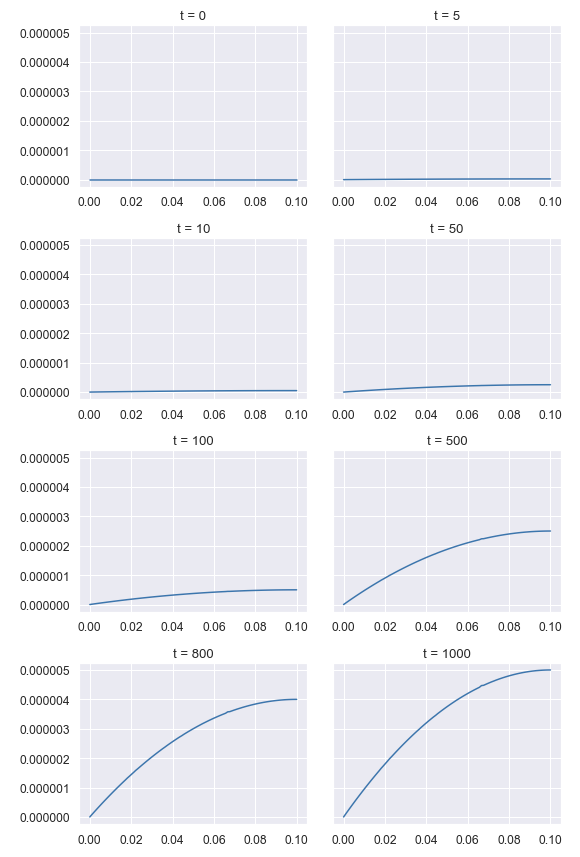
\includegraphics[width=0.8\linewidth]{task2.png}

Как мы видим, задан стержень и на его левом конце в разные моменты времени функция $u$ принимает значение 0. Это верно, поскольку по условию задачи, левый конец стержня зажат. При этом мы видим, что на правом конце функция меняется при изменении времени $t$, что тоже верно, так как правый конец свободен.

\pagebreak